\documentclass[utf8]{beamer}
\usetheme{Antibes}
\usepackage[T1]{fontenc}
\usepackage{tikz}
\usepackage{caption}
\usepackage{url}
\usepackage{listings}
\usepackage{color}

\lstset{
language=python,                % choose the language of the code
basicstyle=\footnotesize,       % the size of the fonts that are used for the code
numbers=left,                   % where to put the line-numbers
numberstyle=\footnotesize,      % the size of the fonts that are used for the line-numbers
stepnumber=1,                   % the step between two line-numbers. If it is 1 each line will be numbered
numbersep=6pt,                  % how far the line-numbers are from the code
backgroundcolor=\color{white},  % choose the background color. You must add \usepackage{color}
showspaces=false,               % show spaces adding particular underscores
showstringspaces=false,         % underline spaces within strings
showtabs=false,                 % show tabs within strings adding particular underscores
frame=L,           % adds a frame around the code
tabsize=2,          % sets default tabsize to 2 spaces
captionpos=b,           % sets the caption-position to bottom
breaklines=true,        % sets automatic line breaking
breakatwhitespace=false,    % sets if automatic breaks should only happen at whitespace
escapeinside={\%*}{*)}          % if you want to add a comment within your code
}

% Postavljanje fonta
\if@fonttimes\RequirePackage{times} \fi
\if@fontlmodern\RequirePackage{lmodern} \fi

\usecolortheme{beaver}
\renewcommand{\figurename}{Slika}

\newcommand{\engl}[1]{(engl.~\emph{#1})}

\title[Projekt]{Izgradnja sufiksnog stabla - Ukkonenov algoritam}
\author{Frane Kurtović i Matija Šantl}

\institute{Bioinformatika\\*Fakultet elektrotehnike i računarstva}
\date{Zagreb, siječanj 2015.}
\begin{document}

\begin{frame}
\titlepage
\end{frame}


\section{Uvod}
\begin{frame}{Uvod}

	Sufiksno stablo \engl{suffix tree} je stablasta struktura podataka koja sadrži sve sufikse nekog niza znakova. 
	
	\vspace{5mm}

	Današnji standard za izgradnju sufiksnog stabla je \textit{Ukkonenov} algoritam iz 1995. godine. To je prvi \textit{on-line} algoritam za izgradnju sufiksnog stabla.
	
\end{frame}

\subsection{Motivacija}
\begin{frame}{Motivacija}

	Ukkonenov algoritam efikasno rješava problem izgradnje sufiksnog stabla, te ima optimalnu (linearnu) vremensku i prostornu složenost. 

	\vspace{5mm}

	Sufiksno stablo na elegantan način rješava problem pretraživanja podniza u nizu, precizinije, podniz je moguće pronaći u vremenu proporcionalnom duljini podniza. 

	\vspace{5mm}

	Također je moguć i pronalazak najduljeg zajedničkog podniza dvaju nizova u vremenu porporcionalnom zbroju njihovih duljina.

\end{frame}

\section{Rezultati}
\begin{frame}{Naslov}
U  nastavku su prikazani razultati za:
\begin{itemize}
	\vspace{5mm}
	\item Escherichia Coli
	\vspace{5mm}
	\item Brochothrix Campestris
	\vspace{5mm}
	\item Sintetički testni primjer
\end{itemize}
\end{frame}

\subsection{Escherichia Coli}
\begin{frame}{Escherichia Coli - vremenska ovisnost}
\begin{figure}[h!]	
	\centering
	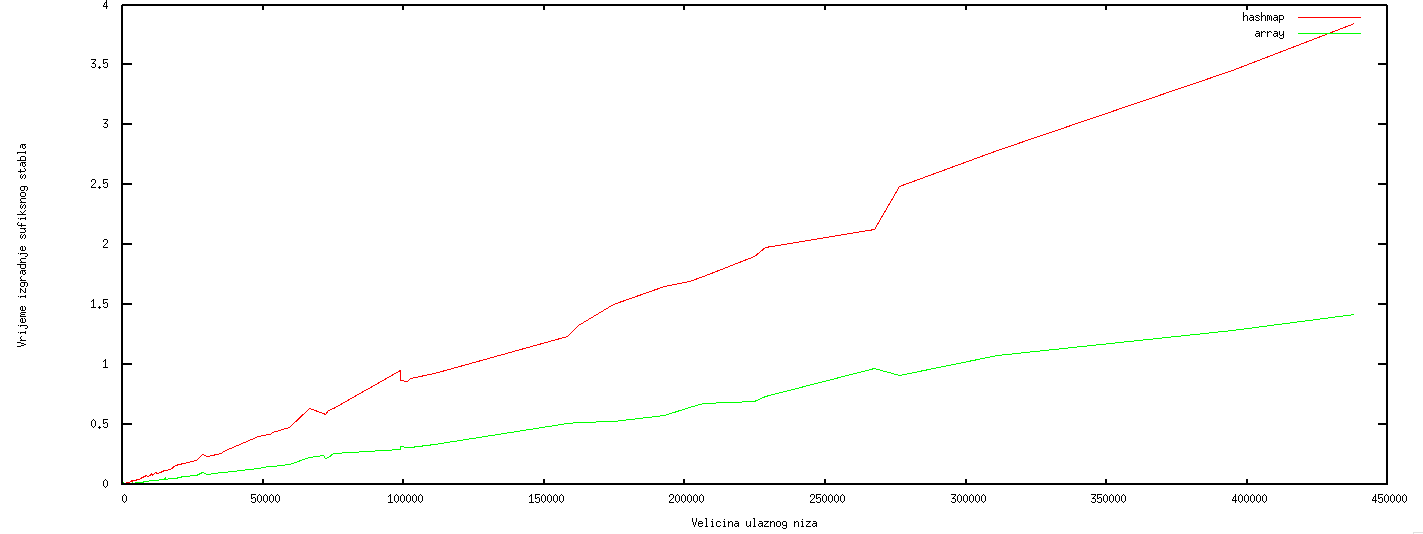
\includegraphics[width=\textwidth]{media/time_1.png}
\end{figure}

\end{frame}
\begin{frame}{Escherichia Coli - prostorna ovisnost}

\begin{figure}[h!]	
	\centering
	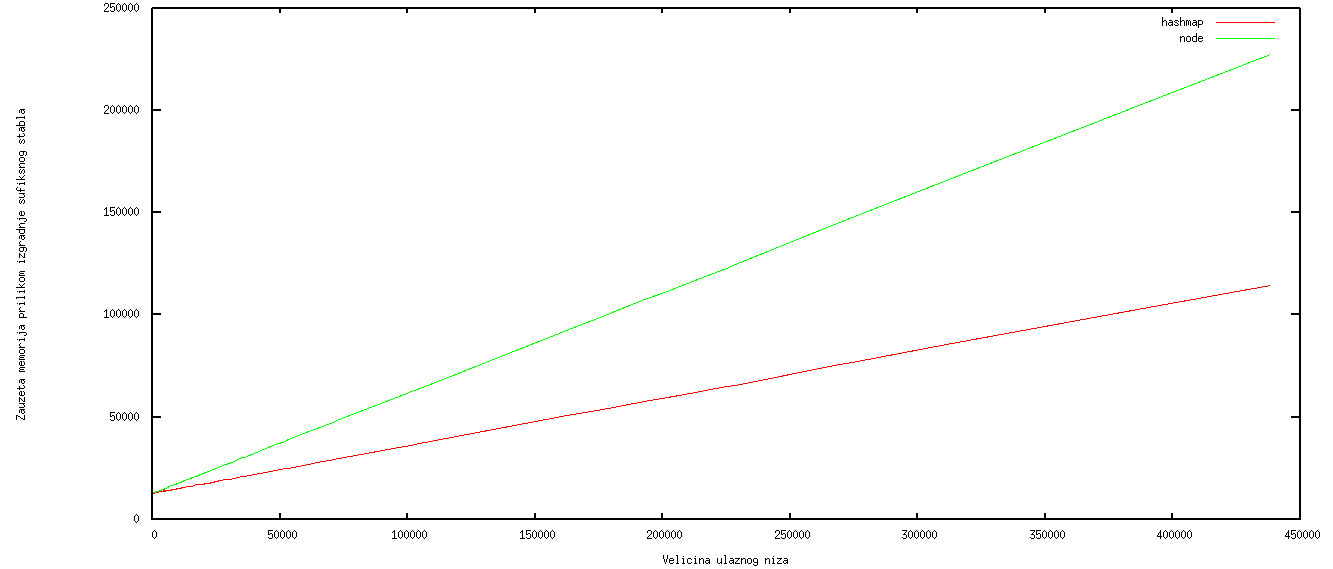
\includegraphics[width=1\textwidth]{media/memory_1.png}
\end{figure}

\end{frame}


\subsection{Brochothrix Campestris}
\begin{frame}{Brochothrix Campestris - vremenska ovisnost}
\begin{figure}[h!]	
	\centering
	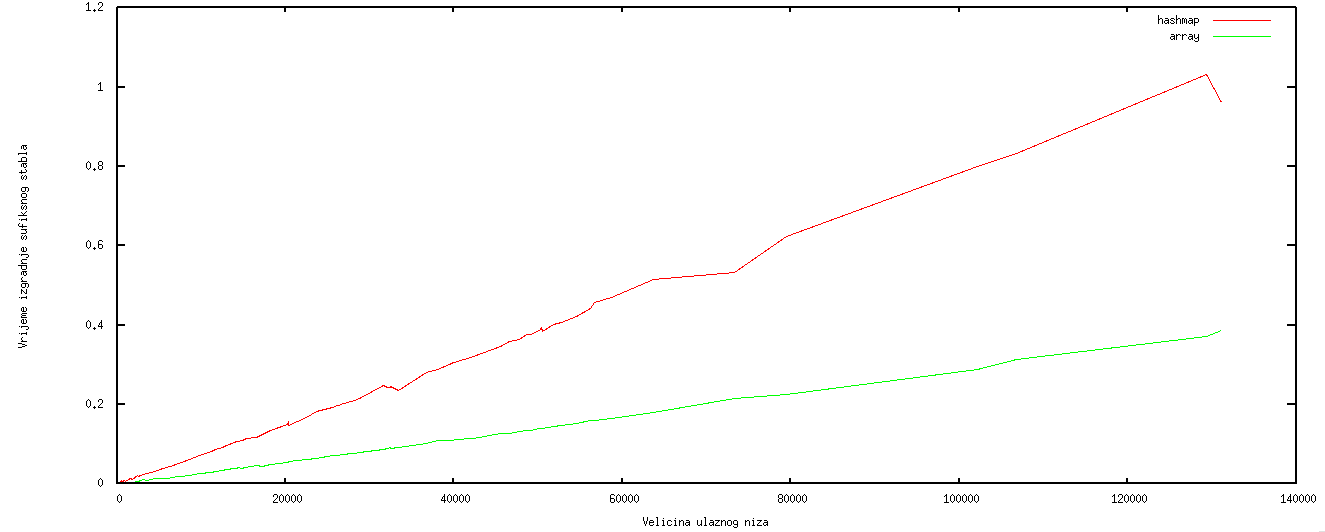
\includegraphics[width=1\textwidth]{media/time_2.png}
\end{figure}

\end{frame}
\begin{frame}{Brochothrix Campestris - prostorna ovisnost}

\begin{figure}[h!]	
	\centering
	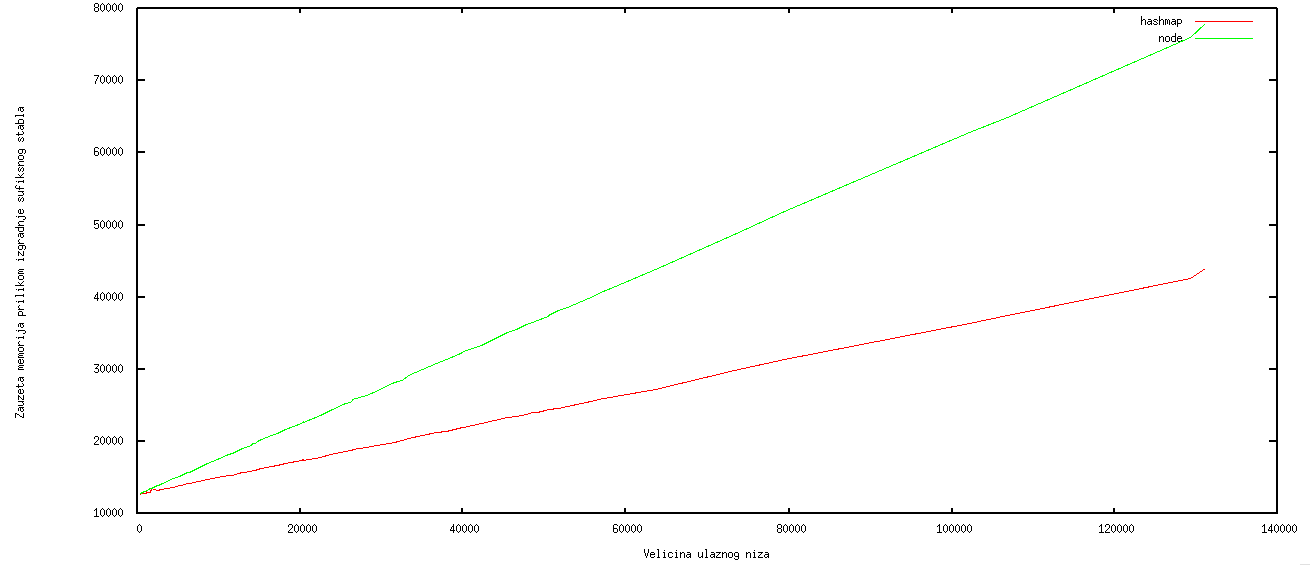
\includegraphics[width=1\textwidth]{media/memory_2.png}
\end{figure}

\end{frame}

\subsection{Sintetički testni primjer}
\begin{frame}{Sintetički testni primjer - vremenska ovisnost}
\begin{figure}[h!]	
	\centering
	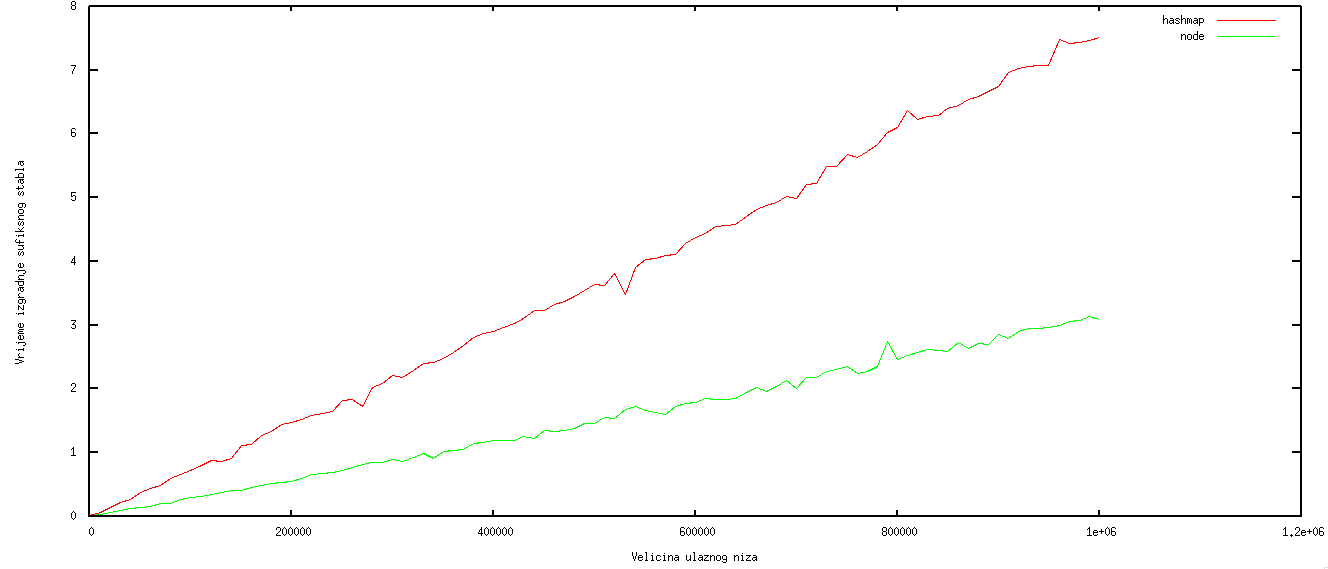
\includegraphics[width=1\textwidth]{media/time_r.png}
\end{figure}

\end{frame}
\begin{frame}{Sintetički testni primjer - prostorna ovisnost}

\begin{figure}[h!]	
	\centering
	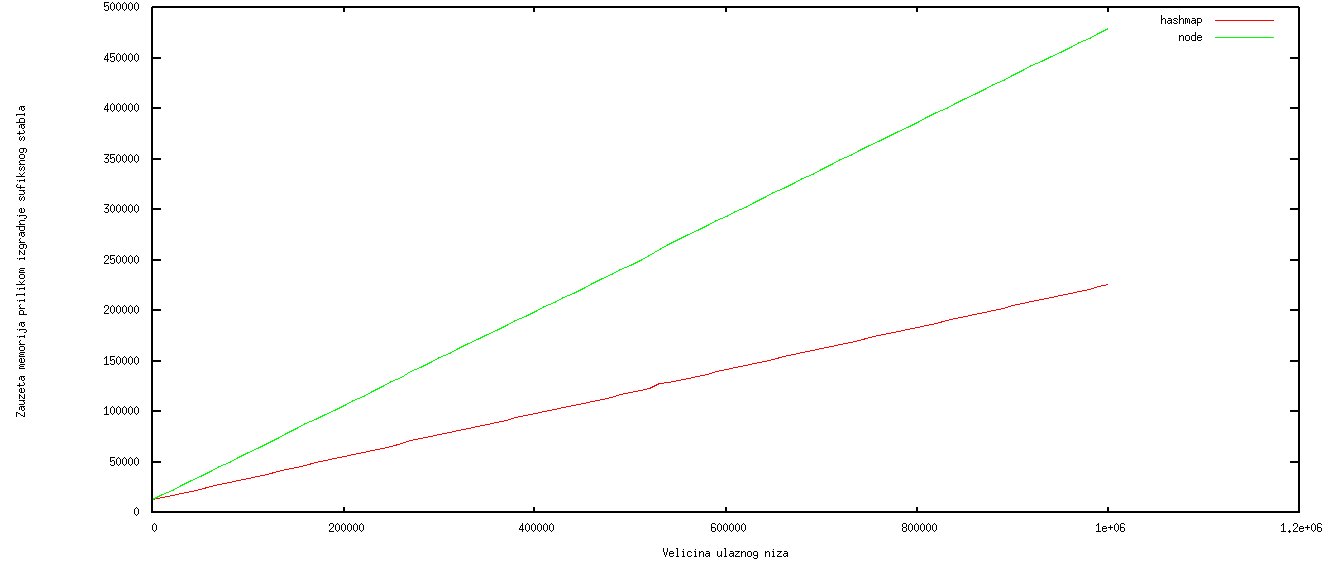
\includegraphics[width=1\textwidth]{media/memory_r.png}
\end{figure}

\end{frame}

\section{Zaključak}
\begin{frame}{Zaključak}

\begin{itemize}
	\vspace{5mm}
	\item vremenska i prostorna složenost izgradnje stabla je linearna s obzirom na duljinu ulaznog niza znakova
	\vspace{5mm}
	\item posjeduje svojstvo procesiranja simbola s lijeva na desno te pritom ima izgrađeno sufiksno stablo za pročitani dio ulaznog niza
\end{itemize}


\pause
\vspace{5mm}
Ostvareno programsko rješenje pokazuje da izgradnja sufiksnog stabla Ukkonenovim algoritmom, i vremenski i prostorno, linearno ovisi o veličini ulaznog niza $T$ .


\end{frame}

\section{Zaključak}
\begin{frame}

\huge{Pitanja?}

\end{frame}

\end{document}